%%%%%%%%%%%
%
% $Autor: Alexandra Roth $
% $Datum: today $
% $Pfad: Montageanleitung.tex $
% $Version: 1.0 $
% !TeX spellcheck = de_DE
% !TeX encoding = utf8
% !TeX TXS-program:bibliography = txs:///biber
%
%%%%%%%%%%%%

\chapter{Montageanleitung Heißdrahtschneidanlage \glqq ELMAR\grqq}


\section{Vorwort: Hinweise zur Fertigung und Montage}

Die Montage der Heißdrahtschneidanlage \glqq ELMAR\grqq{} ist ausschließlich auf sauberen, ebenen Flächen durchzuführen. Alle Werkzeuge, Hilfs- sowie Arbeitsmittel sollten vorab bereitliegen.

Ein Großteil der verbauten Komponenten stammen aus einem Crealitiy Ender 5 Plus 3D-Drucker. Diese Teile sind im Folgenden entsprechend namentlich gekennzeichnet.

Alle 3D-Druck-Teile sind mit den Einstellungen aus dem Bambu Studio-Template zu drucken. Falls ein anderer Slicer (z.B. Ultimaker Cura, Prusa Slicer, Orca Slicer, ...) verwendet wird, sind die Druckeinstellungen gemäß des Bambu Studio Templates zu übernehmen.

Nach dem Druck sind alle Teile auf Qualität und Maßhaltigkeit, sowie alle Funktionsflächen auf Passgenauigkeit zu prüfen. Eventuelle Druckfehler sind zu beheben (z.B. unter dem Einsatz von Feilen) und insbesondere Bohrungen sind sofern nötig auf Sollmaß aufzubohren. Bei Bohrungen, welche zum Einlassen von RUTHEX Gewinde-Einschmelzhülsen vorgesehen sind, ist die Kante zu brechen.

Supportmaterial mit Sorgfalt und vollständig entfernen, z.B. mit Hilfe von Spitzzangen und/oder Pinzetten.

Es wird empfohlen, alle 3d-Druck Teile vorab vor Beginn der Montage vollständig gedruckt, sowie vorbereitet zu haben.

Schrauben und andere Verbindungselemente sind handfest anzuziehen. Ausnahmen davon sind gekennzeichnet.

Zu beklebende Flächen sind vor dem Bekleben falls nötig zu ebnen und anzurauen (z.B. unter Einsatz von Feilen) und mit Isopropanol vorzubereiten. Eine staub- und fettfreie Oberfläche maximiert die Haltbarkeit der Klebung.

Zur besseren Übersicht wurden Normteile (Schrauben, Muttern, Unterlegscheiben) teilweise ausgeblendet. Sie sind außerdem nur an den Stellen explizit genannt, an denen z.B. Verwechslungsgefahr besteht.

Die gesamte Verkabelung geschieht nach Schaltplan.

\section{Werkzeugauswahl}

Folgende Werkzeuge werden benötigt:

\begin{itemize}
	\item Innensechskantschlüssel-Satz
	\item Ringmaulschlüssel-Satz
	\item Schraubendreher
	\item Kunststoffhammer
	\item Lötkolben
	\item Seitenschneider
	\item Spitzzange
	\item Schraubstock
	\item Feilensatz
	\item Messschieber
\end{itemize}

RUTHEX Gewinde-Einschmelzhülsen werden per Lötkolben und mithilfe geeigneter Aufsätze in 3D-Druck-Teile eingeschmolzen. Sie werden grundsätzlich bündig mit der Oberfläche montiert.

\section{Schritt 1: Grundrahmen}

Grundrahmen entsprechend der Montage des Ender 5 Plus miteinander montieren. Dieser besteht aus:

\begin{itemize}
	\item 6x Creality Aluminium-Extrusionsprofil 20 x 20 mm
	\item 4x Creality Aluminium-Extrusionsprofil 40 x 20 mm
	\item 2x Creality Aluminium-Extrusionsprofil 40 x 20 mm, ausgeklinkt
	\item 2x Creality Blech 4 mm für Riemenrolle
	\item 2x Creality Blech 4 mm für Umlenkrolle
	\item 4x Creality Eckwinkel
\end{itemize}

\textbf{ACHTUNG!} Zusätzlich zum Standard-Aufbau müssen noch folgende Komponenten montiert werden.

\begin{itemize}
	\item Druckteil Eckhalter 1
	\item Druckteil Eckhalter 2
	\item 8x Creality Nutenstein
	\item 4x Druckteil Nutenstein-Block
	\item 1x Holzplatte
\end{itemize}

\begin{figure}[htbp]
	\centering
	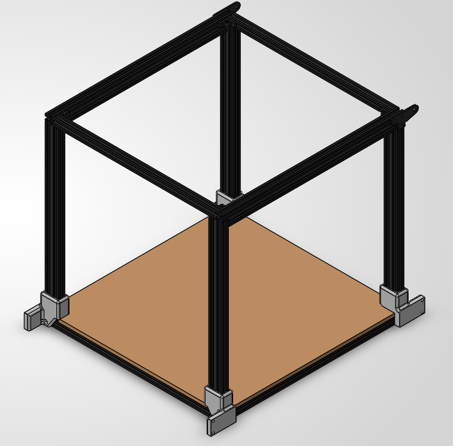
\includegraphics[width=0.65\textwidth]{General/ELMAR_CAD}
	\caption{Grundrahmen der Heißdrahtschneidanlage}
	\label{fig:montage_elmar_cad}
\end{figure}

\section{Schritt 2: Unterbaugruppe Vertikalwagen links}

\begin{itemize}
	\item 2x \glqq 64601006 Linearkugellager KB-3-ST Ø 10\grqq{} in \glqq Druckteil Vertikalwagen links\grqq{} einpressen, z.B. am Schraubstock.
	\item \glqq Spindelmutter\grqq{} verschrauben.
	\item 1x \glqq RUTHEX M5\grqq{} einschmelzen.
	\item \glqq Extruderdüse 0.5 mm\grqq{} einschrauben.
\end{itemize}

\begin{figure}[htbp]
	\centering
	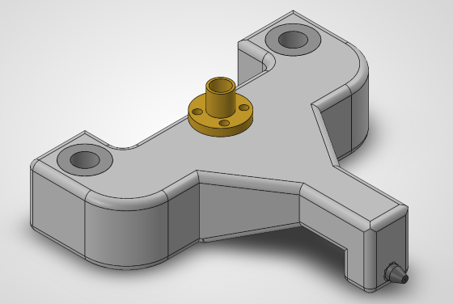
\includegraphics[width=0.58\textwidth]{General/Vertikalwagen_links}
	\caption{Unterbaugruppe Vertikalwagen links}
	\label{fig:montage_vertikalwagen_links}
\end{figure}

\section{Schritt 3: Unterbaugruppe Vertikalwagen rechts}

\begin{itemize}
	\item 2x \glqq 64601006 Linearkugellager KB-3-ST Ø 10\grqq{} in \glqq Druckteil Vertikalwagen rechts\grqq{} einpressen.
	\item 8x \glqq RUTHEX M3\grqq{} in \glqq Druckteil Vertikalwagen rechts (Magazin)\grqq{} einschmelzen.
	\item \glqq Spindelmutter\grqq{} verschrauben.
	\item 1x \glqq RUTHEX M5\grqq{} einschmelzen.
	\item \glqq Extruderdüse 0.5 mm\grqq{} einschrauben.
	\item 1x \glqq Rillenkugellager 12x21x5\grqq{} bündig in \glqq Druckteil Vertikalwagen rechts (Magazin)\grqq{} einpressen.
	\item 4x RUTHEX M4 in \glqq Druckteil Lagerbrücke\grqq{} einschmelzen.
	\item 1x \glqq Rillenkugellager 12x21x5\grqq{} bündig in \glqq Druckteil Lagerbrücke\grqq{} einpressen.
	\item \glqq Druckteil Drahtrolle\grqq{} vorbereiten: Streifen selbstklebender Aluminiumfolie von 7 mm Breite und 750 mm Länge per Schere oder Cutter-Messer und Stahlmaß zuschneiden und auf \glqq Druckteil Drahtrolle\grqq{} aufbringen.
	\item \glqq Heißdraht\grqq{} 3 Mal um die \glqq Fixierungsschraube\grqq{} wickeln, dann durch die Führungsnut führen und 3 Mal um \glqq Druckteil Drahtrolle\grqq{} wickeln, das freie Ende von innen nach außen durch die \glqq Extruderdüse 0.5 mm\grqq{} führen. \textbf{ACHTUNG!} Knicken des Heißdrahtes unbedingt vermeiden!
	\item \glqq Flachspiralfeder\grqq{} in die Nut auf der Rückseite der \glqq Druckteil Drahtrolle\grqq{} setzen und fixiert halten.
	\item Fertig vorbereitete \glqq Druckteil Drahtrolle\grqq{} in \glqq Druckteil Vertikalwagen rechts (Magazin)\grqq{} einsetzen, dabei die \glqq Flachspiralfeder\grqq{} auf der Arretierungsschraube aufliegen lassen.
	\item \glqq Druckteil Lagerbrücke\grqq{} mitsamt vormontiertem \glqq Rillenkugellager 12x21x5\grqq{} über freies Ende von \glqq Druckteil Drahtrolle\grqq{} stecken, am \glqq Druckteil Vertikalwagen rechts (Magazin)\grqq{} verschrauben.
\end{itemize}

\begin{figure}[htbp]
	\centering
	\begin{minipage}{0.48\textwidth}
		\centering
		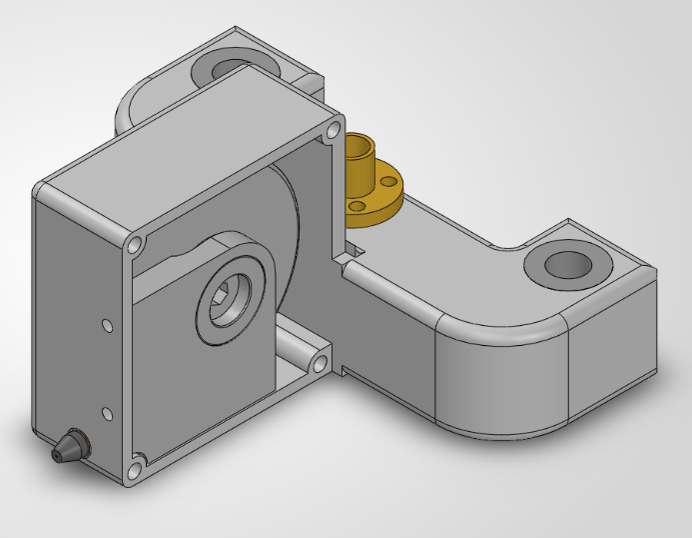
\includegraphics[width=\linewidth]{General/Vertikalwagen_rechts}
		\caption{Vertikalwagen rechts}
		\label{fig:montage_vertikalwagen_rechts}
	\end{minipage}
	\hfill
	\begin{minipage}{0.48\textwidth}
		\centering
		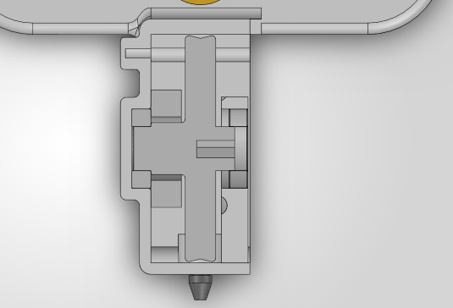
\includegraphics[width=\linewidth]{General/Vertikalwagen_rechts_unten}
		\caption{Vertikalwagen rechts, Unterseite}
		\label{fig:montage_vertikalwagen_rechts_unten}
	\end{minipage}
\end{figure}

\section{Schritt 4: Vormontage Unterbaugruppe Horizontalwagen (2x)}

\begin{itemize}
	\item 14x RUTHEX M3 und 2x RUTHEX M5 in \glqq Druckteil Führung oben, Teil 1\grqq{} einschmelzen.
	\item \glqq Druckteil Führung oben, Teil 1\grqq{} mit \glqq Druckteil Führung oben, Teil 2\grqq{} wie unten gezeigt (blau markiert) mit Senkschrauben M3x12 vorverschrauben.
	\item \glqq Creality Trägerplatte\grqq{} bis zum Anschlag in vormontierte Baugruppe einschieben.
	\item Verschraubung von \glqq Druckteil Führung oben, Teil 1\grqq{} mit \glqq Druckteil Führung oben, Teil 2\grqq{} mit M3x16, M5x12, M5x16 komplettieren, dabei \glqq Stepper Motor\grqq{} verschrauben (Linsenkopfschrauben M3x18).
	\item \glqq Creality Rolle mit Lager\grqq{} (4x), \glqq Creality Abstandhülse für Rolle mit Lager\grqq{} (4x) und \glqq Exzentermutter\grqq{} (2x) montieren.
	\item \glqq Creality Kupplung\grqq{} und \glqq Creality Leitspindel TR8x2\grqq{} montieren.
	\item \glqq Creality Führungsstahl vertikal\grqq{} bis zum Anschlag in \glqq Druckteil Führung oben, Teil 2\grqq{} per Kunststoffhammer einschlagen.
	\item \textbf{ACHTUNG! RICHTUNG BEACHTEN:} \glqq Druckteil Endschalter-Halter rechts\grqq{} bzw. \glqq Druckteil Endschalter-Halter links\grqq{}, \glqq Creality Endschalter\grqq{} und \glqq Druckteil igus Adapter rechts\grqq{} bzw. \glqq Druckteil igus Adapter links\grqq{} anschrauben.
\end{itemize}

\begin{figure}[htbp]
	\centering
	\begin{minipage}{0.32\textwidth}
		\centering
		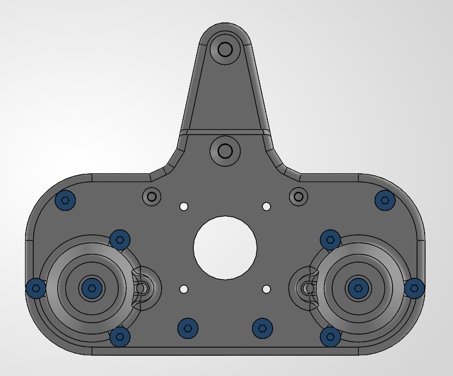
\includegraphics[width=\linewidth]{General/Horizontalwagen}
		\caption{Horizontalwagen}
		\label{fig:montage_horizontalwagen}
	\end{minipage}
	\hfill
	\begin{minipage}{0.32\textwidth}
		\centering
		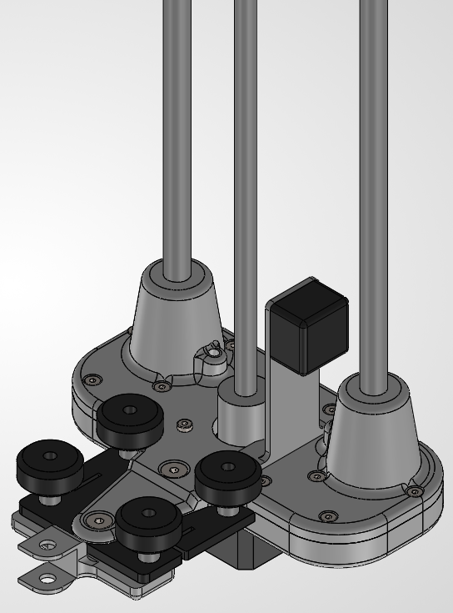
\includegraphics[width=\linewidth]{General/Horizontalwagen_montiert}
		\caption{Horizontalwagen montiert}
		\label{fig:montage_horizontalwagen_montiert}
	\end{minipage}
	\hfill
	\begin{minipage}{0.32\textwidth}
		\centering
		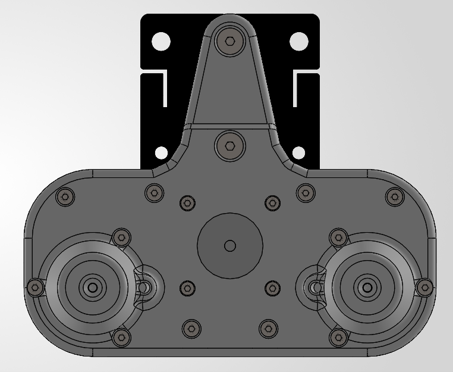
\includegraphics[width=\linewidth]{General/Horizontalwagen2}
		\caption{Horizontalwagen, weitere Ansicht}
		\label{fig:montage_horizontalwagen_2}
	\end{minipage}
\end{figure}

\section{Schritt 5: Fügen Horizontalwagen mit Vertikalwagen links / rechts}

\begin{itemize}
	\item 4x RUTHEX M4 in \glqq Druckteil Führung unten\grqq{} einschmelzen.
	\item \glqq Unterbaugruppe Vertikalwagen links\grqq{} und \glqq Unterbaugruppe Vertikalwagen rechts\grqq{} jeweils auf eine vormontierte Unterbaugruppe Horizontalwagen aufstecken.
	\item Die freien Enden der jeweils beiden \glqq Creality Führungsstahl vertikal\grqq{} in \glqq Druckteil Führung unten\grqq{} bis Anschlag einschlagen, per Kunststoffhammer.
	\item \glqq Creality Linearführung rund\grqq{} (2x pro Seite) an \glqq Druckteil Führung unten\grqq{} verschrauben.
\end{itemize}

\begin{figure}[htbp]
	\centering
	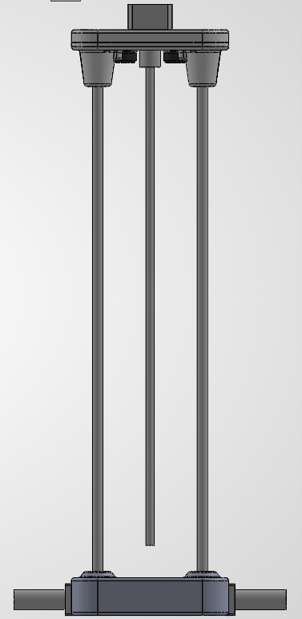
\includegraphics[width=0.55\textwidth]{General/Vertikalwagen_und_Horizontalwagen}
	\caption{Gefügter Vertikalwagen mit Horizontalwagen}
	\label{fig:montage_vertikalwagen_und_horizontalwagen}
\end{figure}

\section{Schritt 6: Fügen mit dem Rahmen}

Beide Baugruppen aus jeweils Horizontal- und Vertikalwagen mit den \glqq Creality Rollenmit Lager\grqq{} oben am Rahmen (explizit: Creality Aluminium-Extrusionsprofil 40 x 20 mm, ausgeklinkt) einhängen.

\section{Schritt 7: Führung unten}

\glqq Creality Führungsstahl horizontal\grqq{} durch \glqq Creality Linearführung rund\grqq{} führen und mit \glqq Creality Klemme für Führungsstab\grqq{} über \glqq Druckteil Eckhalter 1\grqq{} bzw. \glqq Druckteil Eckhalter 2\grqq{} am Rahmen befestigen.

\glqq Creality Rollen mit Lager\grqq{} oben am Rahmen so einstellen, dass wenig spiel auftritt, während Leichtläufigkeit der Achse gegeben ist.

\section{Schritt 8: Motoren, Endschalter, Energieketten, Riemen und Schneidematte}

Folgende Teile werden in diesem Schritt verbaut:

\begin{itemize}
	\item Endschalter-Halter oben
	\item Creality Endschalter
	\item Blech 3 mm Motorwinkel hinten
	\item Stepper Motor
	\item Creality Kupplung
	\item Creality Welle 8 mm
	\item Creality Riemenrolle
	\item Creality Abstandhülse für Riemenrolle
	\item Druckteil igus Adapter Rahmen links
	\item Energiekette
	\item Creality Umlenkrolle
	\item Creality Blech 4 mm für Umlenkrolle
\end{itemize}

Den Riemen durch das \glqq Creality Aluminium-Extrusionsprofil 40 x 20 mm, ausgeklinkt\grqq{} führen, um die \glqq Creality Umlenkrolle\grqq{} und \glqq Creality Riemenrolle\grqq{} herum, und in der \glqq Creality Trägerplatte\grqq{} einspannen. Die Riemenspannung mit der Umlenkrolle einstellen. Sollte es im Betrieb zum überspringen des Riemens kommen, kann hier die Riemenspannung erhöht werden. Sollte die Achse besonders schwerfällig sein, kann sehr hohe Riemenreibung durch Riemenspannung ein Auslöser sein. In diesem Fall kann diese hier reduziert werden.

Die Bilder zeigen die linke Rahmenseite. Auf der rechten wird ein hierzu symmetrischer Aufbau benötigt. \textbf{ACHTUNG:} Die Energieketten sind hier nur schematisch angedeutet.

\begin{figure}[htbp]
	\centering
	\begin{minipage}{0.48\textwidth}
		\centering
		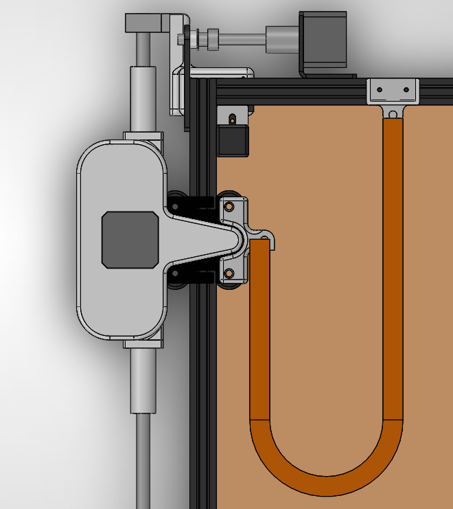
\includegraphics[width=\linewidth]{General/Rahmenseite_links}
		\caption{Rahmenseite links}
		\label{fig:montage_rahmenseite_links}
	\end{minipage}
	\hfill
	\begin{minipage}{0.48\textwidth}
		\centering
		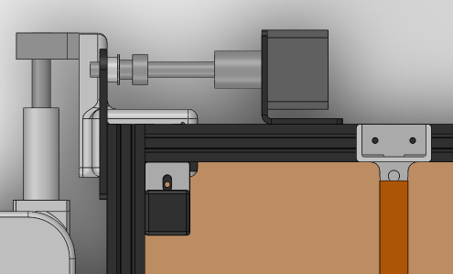
\includegraphics[width=\linewidth]{General/Rahmenseite_links_oben}
		\caption{Rahmenseite links, obere Ansicht}
		\label{fig:montage_rahmenseite_links_oben}
	\end{minipage}
\end{figure}

\section{Schritt 9: Heißdraht spannen}

In \glqq Druckteil Drahtrolle\grqq{} befindet sich die Aufnahme für einen Innensechskantschlüssel (5 mm). Dieser wird genutzt, um die Rolle auf Federspannung zu halten, während das noch freie Ende des Heißdrahtes nun durch die Extruderdüse auf der linken Seite geführt, und dahinter verknotet wird. Es wird empfohlen, ca. 2,5 der 3 Draht-Umdrehungen beim Spannen der Flachspiralfeder abzuwickeln, um die korrekte Drahtspannung zu gewährleisten. Eine zu hohe Drahtspannung übt hohe Belastungen auf alle mechanischen Komponenten, insbesondere im Bereich der Vertikal- und Horizontalwagen aus, ein zu geringe Drahtspannung kann dazu führen, dass der Draht nicht ordnungsgemäß durch die Extruderdüse auf der rechten Seite zurückgezogen wird.

Ist die Drahtspannung korrekt eingestellt, kann das \glqq Druckteil Abdeckkappe\grqq{} verschlossen werden.

\begin{figure}[htbp]
	\centering
	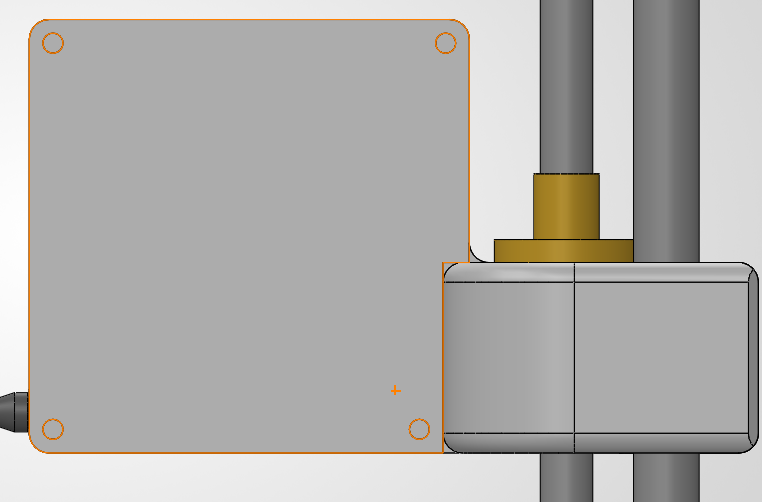
\includegraphics[width=0.55\textwidth]{General/Abdeckkappe}
	\caption{Abdeckkappe der Drahtrolle}
	\label{fig:montage_abdeckkappe}
\end{figure}
